\section{Results}

We started with a TensorFlow model of 98.43\% accuracy. Using the techniques described in this document together with the cryptographic algorithm the accuracy achieved was 98.40\%, ie only 0.03\% less than the base model. But the processing times were long, longer than those obtained in the original paper. To run tests on a set of 10,000 images, we spent 6 hours on a PC with a single Intel Core i7-4820K CPU running at 3.7GHz, with 12GB of RAM, running the Ubuntu 18.04 operating system. Of these 6 hours, 4 are used by the first layer only. But the time is to be divided between the phases of encoding, encrypting and the application of the neural network. The decoding and decrypting phases turned out to be very fast. Applying the network allows making chunks of 4096 predictions simultaneously, so the actual time taken by an image to be encoded, encrypted and transformed into prediction is less than 2 seconds. A speed equal to about 2048 predictions per hour has thus been obtained. Ie, about one eighth of the speed obtained in \cite{dowlin2016cryptonets}: in the original project 10000 instances are classified in 2263.5 seconds, that is, they reached a speed equal to 15904.6 predictions per hour. The fact that our speed is an eighth of theirs by using a PC with similar characteristics is no coincidence, and should not surprise. In that project, the algorithm used is YASHE, in which a polynomial in $R^n_t$ is transformed into a single polynomial in $R^n_q$. In our case instead, due to the new version of the SEAL library, a polynomial in $R^n_t$ is transformed into an array of polynomials in $R^{n+1}_q$, where the array has two elements, and each element is a set of four polynomials, one for each $q_i$, for a total of 8 polynomials of degree $n+1$. The size of the data to be processed is therefore eight times higher. However, it should be noted that each coefficient of the encrypted message in our case is a 64-bit unsigned variable, while in the original CriptoNets project it is 192 bits. Our algorithm should therefore be three times faster than what we actually got. This did not happen probably due to some differents such as the particular specifics in the PC used. But mostly due to the programming language chosen: the original project was in fact written entirely in the C++ programming language, while we chose to use Python for ease of use. Moreover, part of the time spent was used to save the tensor outputs after each layer and, since the tensors can be very large, this process takes time. The files obtained are in fact very large, and for this reason they have not been uploaded to github:

\begin{center}
\begin{tabular}{ |c|c|c| } 
\hline
File name & Tensor size & File size \\
\hline
\hline
\texttt{enc_layer_0.npy} & (98328, 29, 29, 5) & 3,308 MB \\
\texttt{enc_layer_1.npy} & (98328, 845, 5) & 3,323 MB \\
\texttt{enc_layer_2.npy} & (98328, 845, 5) & 3,323 MB \\
\texttt{enc_layer_3.npy} & (98328, 100, 5) & 466 MB \\
\texttt{enc_layer_4.npy} & (98328, 100, 5) & 393 MB \\
\texttt{enc_layer_5.npy} & (98328, 10, 5) & 47 MB \\
\hline
\end{tabular}
\end{center}

Finally, we need to consider the to_object_dtype() function which, as we found, although necessary for using the NumPy .dot() operator, it also require quite some time. To conclude, we highlight the size of the messages. The messages to be exchanged between the data owner and the cloud for a single chunk of 4096 images are therefore 1103 MB (for the images) and 16 MB (for the predictions).

\begin{figure}[H]
	\centering
	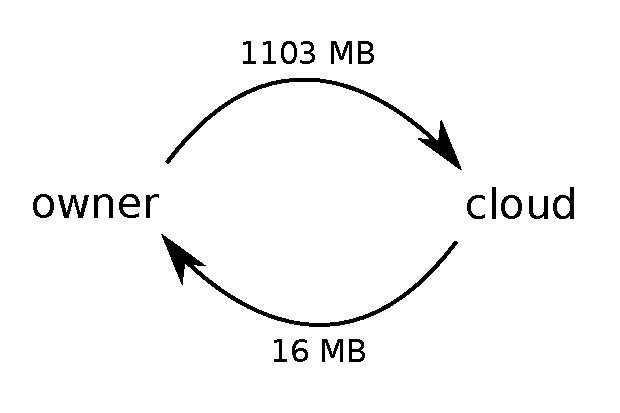
\includegraphics[width=0.5\textwidth]{images/fig5.pdf}
    \caption{Messages exchanged between the owner and the cloud.}
    \label{fig:im4}
\end{figure}
